\chapter{Testing}
\label{chap:Testing}

Testing is an integral part of software development for any system. Testing is done to ensure that the product delivered at the end of the development process actually functions as intended. However, the number of errors in any software can be quite large and even with extensive testing, faults and bugs can still be undetected. To address this issue it is important to conduct tests that examine the core functionalities as decided upon in collaboration with the customer, and specified by both the system requirements as well as the use cases.

\paragraph{} Additionally the quality requirements must be tested, since these requirements are not simply a matter of correct response to stimulus but rather a degree of acceptability. Quantifying them can be a difficult process, especially as tolerance levels for specific factors are subjective and vary between persons (\cite{website:software-testing-Jiantao-Pao}). In section \ref{sec:TestingMethods} we give a brief introduction of the different testing methods used during development, while we in section \ref{sec:TestingApproach} describe how the actual testing was performed.

\newpage
\section{Test Methods}
\label{sec:TestingMethods}

\subsection{Black Box} 
\label{subsec:TestingMethodBlack}
A black box test is a test in which the end functionalities of a system is tested, the test person is not concerned with how the program processes information, only if the end result of the process is correct. As such the test may be designed and carried out by people without knowledge of the underlying code of the system. By having a person without knowledge of the code designing the test, the test can detect faults that the developer might have considered too obvious to handle or respond to properly, and get a different perspective on what the most important features of the system are. On the other hand a person without knowledge may create redundant test that end up testing the same underlying set of functions, while other parts of the source code may not be tested at all. \cite{book:software-testing-Patton}

\begin{figure}[ht!]
\centering
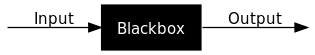
\includegraphics[width=90mm]{./Testing/img/BlackBoxTesting.png}
\caption{The Black Box process. \label{TestBB}}
\end{figure}

\subsection{White Box}
\label{subsec:TestingMethodsWhite}
White box testing refers to tests that are made on a source code level. A white box test is made with knowledge of what part of the source code is responsible for which functionalities, and the relevant code is then tested to see if it provides correct feedback. White box testing is a good method for testing existing code for faults, but because the tests only operate on implemented code this method is unable to detect missing functionalities. By knowing what parts of the code is involved in testing, a white box text is able to pinpoint the defect code with much more accuracy than a black box test. \cite{article:forms-of-software-testing,website:white-box-testing}

\subsection{Gray Box}
\label{subsec:TestingMethodsGray}
The gray box test method combines the black and white box methods by utilizing source code knowledge while designing test that are intended to be executed on the user level like a black box test. The gray box method is aimed at finding defects resulting from improper use of applications, or from improper structure. As the gray box approach utilizes some background knowledge it is suitable for functional testing. \cite{inproc:gray-box}

\section{Testing Approach}
\label{sec:TestingApproach}

In this project, testing was done continually during development. In the most basic form this testing consisted of attempting to execute the code and trying to trace faults and then correct the code. This process was made easier by the use of built in proofreading functions in the code editor. All of these test are performed for every newly added feature. This kind of testing could have been automated by writing unit tests executed with unit testing software, but since we were only developing a prototype, we chose to not spend time doing so.

\paragraph{} In addition to the ongoing code correction and checking, new components and features that had been completed and cleared, were integration tested both to ensure correct behaviour of the new functionalities, and to check for unintentional faults caused in the rest of the system. The code checks and corrections, as well as the integration tests were all white box tests performed by the developers to ensure that the code was working properly. The aforementioned tests were all intended to ensure that the program behaved correctly. In order to verify that the actual functionality of the program matched the intended functionality as agreed upon with the customer, functional tests were designed based on the requirements of the system. The test cases for the functional tests are detailed in appendix \ref{chap:TestingTPlan}. %\ref{chap:TestPlan} 

\section{System Test}
\label{sec:TestingSystem}

When the prototype were considered finished with all agreed functionality, a complete system test were conducted. Here all of the designed functional tests were executed  in order to ensure that all functionality was working as expected. This was done by the team members with least implementation involvement, to prevent avoidance of known bugs, if any present. The results from the system test are detailed in appendix \ref{chap:TestingTPlan}. As seen in the test results, a couple of bugs did appear when performing the test. Those bugs were looked into and fixed by the development team. In the following section the outline of the test cases are described.

\subsection{Test Case Overview}
\label{subsec:TestingSystemOverview}
In order to keep track of the different test cases, all cases got assigned an unique identifier. All of these identifiers were written on the following form: FTXX. FT stands for functional test, while XX stands for the number of the test. In table \ref{TestingStandard} the template used for writing test cases can be viewed. \\ \\ 
%
\begin{minipage}{\linewidth}
\setlength{\tabcolsep}{15pt}
\centering
\rowcolors{1}{blue!20}{blue!10}
\begin{tabular}{ |l|p{70mm}| }
	\hline
	\it{\cellcolor{gray!25}Item} & {\cellcolor{gray!25} Description } \\
	\hline
	\it{\cellcolor{gray!25}Test Name } & The name of the test.  \\ \hline
	\it{\cellcolor{gray!25}Test ID} & The test identifier  \\ \hline
	\it{\cellcolor{gray!25}Feature to be tested} & What functionality will be tested.  \\ \hline
	\it{\cellcolor{gray!25}Requirements} & Which requirements this test is related to.  \\ \hline
	\it{\cellcolor{gray!25}Pre-conditions} & Fullfilled conditions we assume to be working when performing the test.  \\ \hline
	\it{\cellcolor{gray!25}Steps of Execution} & Steps of how the test should be carried out.  \\ \hline
	\it{\cellcolor{gray!25}Steps of Execution} & The expected results from the steps above.  \\
	\hline
\end{tabular}
\captionof{table}{Standard table used for documenting test cases in the appendix. \label{TestingStandard}}
\end{minipage}

\section{Non-functional Requirements Testing}
\label{sec:TestingNRT}

Although testing of required functionality is important when developing software, testing of non-functional requirements are equally important. In the system requirements section of this report we lists requirements for usability, performance, security, availability and scalability as this systems non-functional requirements. When developing the final version of this system, all of those requirements are essential for achieving a well functioning system. In the prototype we have been developing, we chose to specifically pursue one of those, namely the usability requirements. The reasoning behind this, were that the prototype were meant to show off essential functionality and how it could be intuitively used. That way our customer could hopefully reach their goal of further funding, to realize a fully functional consumer version of the system. 

\subsubsection{Usability} Usability can be described as how easy a human made object is to use and learn. In our case, this means the ease of use of our website and mobile app. Is the website visually appealing and intuitive? Is it easy to understand what one can do on the website and what functionality it provides? Are the common functions behaving as expected? When testing the usability of our system all of these questions were taken into account.

\paragraph{} From the ISO [9241]  definition of usability we have that the usability of a product is:
“The extent to which a product can be used by specified users to achieve specified goals with effectiveness, efficiency, and satisfaction in a specified context of use". As mentioned earlier, quantifying or measuring the usability of a system can be difficult, as it often come down to subjective preferences and opinions. Therefore we needed to find out what effectiveness, efficiency, and satisfaction meant in our system.

\subsubsection{Effectiveness} To measure the effectiveness of our website and mobile app, it made sense to base this upon the number of tasks an end user were able to complete without assistance within a specific timeframe. The higher the number of completed tasks, less time was spent wondering how to do something, resulting in a more effective user. 

\subsubsection{Efficiency} The efficiency measurement were based upon the time spent performing some task on the website or mobile app.The smaller the amount of time spent performing some task, the higher the possibility for the user to want to perform it again.Whenever some function takes too long time, the user might find the process both tedious and boring, and will possibly refrain from using the function later.

\paragraph{Satisfaction} Measuring the level of satisfaction of using the website or mobile app was the most challenging part when measuring the overall usability. We chose to base the measurement on oral feedback from the test users.

\subsubsection{Usability Testing} The actual execution of the usability testing were divided into two categories. One being testing within the group, and the second being testing with actual end users. The testing within the group was an ongoing process throughout the duration of development, while testing with end users was a one time thing. Below follows a more detailed description of what we decided to test and how the tests should be performed, before going into details of how testing within the group and with the end users were conducted.

\subsubsection{What to Test} The main goal with the usability tests is to examine whether the functionality of the website is easy to learn and use, as well as the understanding of the main concept. Being a website centered around a 2-dimensional image and event search, it is specifically important to get an understanding of how intuitive that functionality appears. Will the test persons understand that the map can be used to change the search results? How easy will they find it to navigate the map? How about the the interest search bar? Will they find it, and understand how it is used?

\paragraph{} As well as getting feedback about the core functionality, we want to use the tests to detect different bugs and errors. This can be bugs showing up as a cause of using the website differently than what is intended, or errors being caused by unexpected input values. Therefore all forms and different input fields should be tested thoroughly.

\paragraph{} Lastly, we want to find out if there is something about the overall design or coloring that should be changed. This can be text being hard to read, caused by an unfortunate text- or background color choice, or elements that is too big or too small.  

\subsubsection{Test execution} Before starting the test, the test person will get a brief explanation of the test process by the group member who created the test. The website will then be loaded and the test person given tasks to perform while being encouraged to think aloud. When all tasks are completed, the test person will be asked to provide an overall opinion of the website, as well as an explanation of the general experience.

\subsubsection{Group testing}
As mentioned earlier the usability of both the website and mobile app were continuously tested within the group. This testing involved group members trying out newly added features on their own, and providing feedback to the rest of the group at group meetings. This feedback could be suggestions to improve navigation between different pages, coloring of different UI elements, and so on. When functionality appeared hard to understand or tedious to do, the group was informed and actions were made. Even though we tested and improved the usability continuously, no formal tests were executed regarding usability during development. The reason for this was that with such a limited time frame, executing these tests on a regular basis would take up too much time that could be spent on further development. We also found the non-formal tests to be very valuable.

\subsubsection{User testing}
In order to get user feedback on our system, two group members traveled to T{\o}yen in Oslo. Here they met up with possible end-users, at a house for youth called “Riverside”. Some of the youth currently at the house, were asked to try out our website, while one group member who created the test and the other monitored and took notes. The tests were conducted following the test execution described above. The member who created the tests gave instructions of what the test person should do, and then letting the test person perform the given tasks without assistance. During all of the tests, the test persons were asked to explain their thought process. That way it was easier to understand what functionality of the website that could be confusing, hard to understand or tedious, and also what functionality that worked well. At the end of the tests, the test persons were asked to give their overall opinion of the website. Even though no timing or counting of the performed tasks were done, we got a clear understanding of the effectiveness, efficiency and satisfaction of our website at the current stage of development. The results from these tests can be found in Appendix~\ref{chap:TestingResults}, more information about the trip to Oslo and general feedback from the end users can be found in section \ref{sec:S2Presentation}.